% Document class `report-template` accepts either project-plan or final-report option in [].
\documentclass[final-report]{report-template}

% Packages I use in my report.
\usepackage{graphicx}
\usepackage{amsmath}
\usepackage{blindtext}
\usepackage{float}

% Directory where I saved my figures.
\graphicspath{{./figures/}}

% Metadata used for the title page - please modify.
\university{Imperial College London}
\department{Department of Earth Science and Engineering}
\course{MSc in Environmental Data Science and Machine Learning}
\title{Building a route optimization system that takes elevation into consideration}
\author{Jinsong Dong}
\email{jinsong.dong22@imperial.ac.uk}
\githubusername{edsml-jd622}
\supervisors{Sesinam Dagadu\\
             Dr. Yves Plancherel}
\repository{https://github.com/ese-msc-2022/irp-jd622}

\begin{document}

\maketitlepage  % generate title page

% Abstract
\section* {Abstract}
Urban traffic planning and route optimization in real-world road networks are crucial for efficient transportation systems. 
This study presents a multifaceted approach to address these challenges. 
It introduces a tool capable of integrating 2D road data with elevation information, 
effectively creating a 3D representation of road networks. 
The tool also offers route planning and visualization capabilities.

The integration function can be applied to any user-specified region. 
When it comes to route planning, 
the tool achieves a relative error of 11.95\% in finding the shortest path and 23.73\% in determining the most time-efficient route, 
compared to Google Maps.

To extend its utility, the study delves into solving the Traveling Salesman Problem (TSP) within real-world street networks. 
A modified Pointer Network is implemented, which can predict TSP solutions from adjacency matrices. 
This model exhibits an accuracy rate of 67.0\%, with an average route length ratio of 1.02 concerning optimal route length.

The combination of these advancements offers a robust solution for urban traffic planning, 
incorporating terrain considerations and real-world road network complexities. 
This research lays the groundwork for more efficient and sustainable transportation systems in urban areas.

% Introduction section
\section {Introduction}
\subsection {Route optimization problem}
A route optimization problem for real-world road networks can be divided into two parts generally.
The first part is finding the shortest path problem, 
which is finding a path between two intersections on a road map such that the sum of the distance of the constituent road is minimized.
For this part, the famous Dijkstra's algorithm\cite{Dijkstra:1959aa} based on the graph theory is already a mature method.
But Dijkstra can only solve the single-source shortest path problem with non-negative edge weight.
The Bellman-Ford algorithm\cite{bellman} can deal with the shortest path problem with negative edge weight, 
but it is slower than the Dijkstra algorithm.
Some research has been done to improve the computing efficiency of these algorithms\cite {journals/tpds/BusatoB16}.
For a road network, distance is a non-negative weight, so the Dijkstra algorithm is a better choice.

The second part is making route optimization. 
The route optimization problem in this project is a kind of Travel Salesman Problem(TSP) \cite{lawler1985travelling}, 
which means given a list of cities and distances between each pair of cities, what is the shortest possible
route that visits each city exactly once and returns to the origin city \cite{TSP_wiki}. 
TSP is a classic NP-hard problem, which means it can not be solved in polynomial time.
One example of a solution of a TSP is shown in Fig.~ \ref{fig:solution_of_TSP}.
In this example, there are 35 locations in total, and the shortest way between these locations is drawn in the line.
There are $35!$ possible combinations of the route total, the 'brute-force solution' will take a very long time to get the results.
\begin{figure}[H]
    \begin{center}
        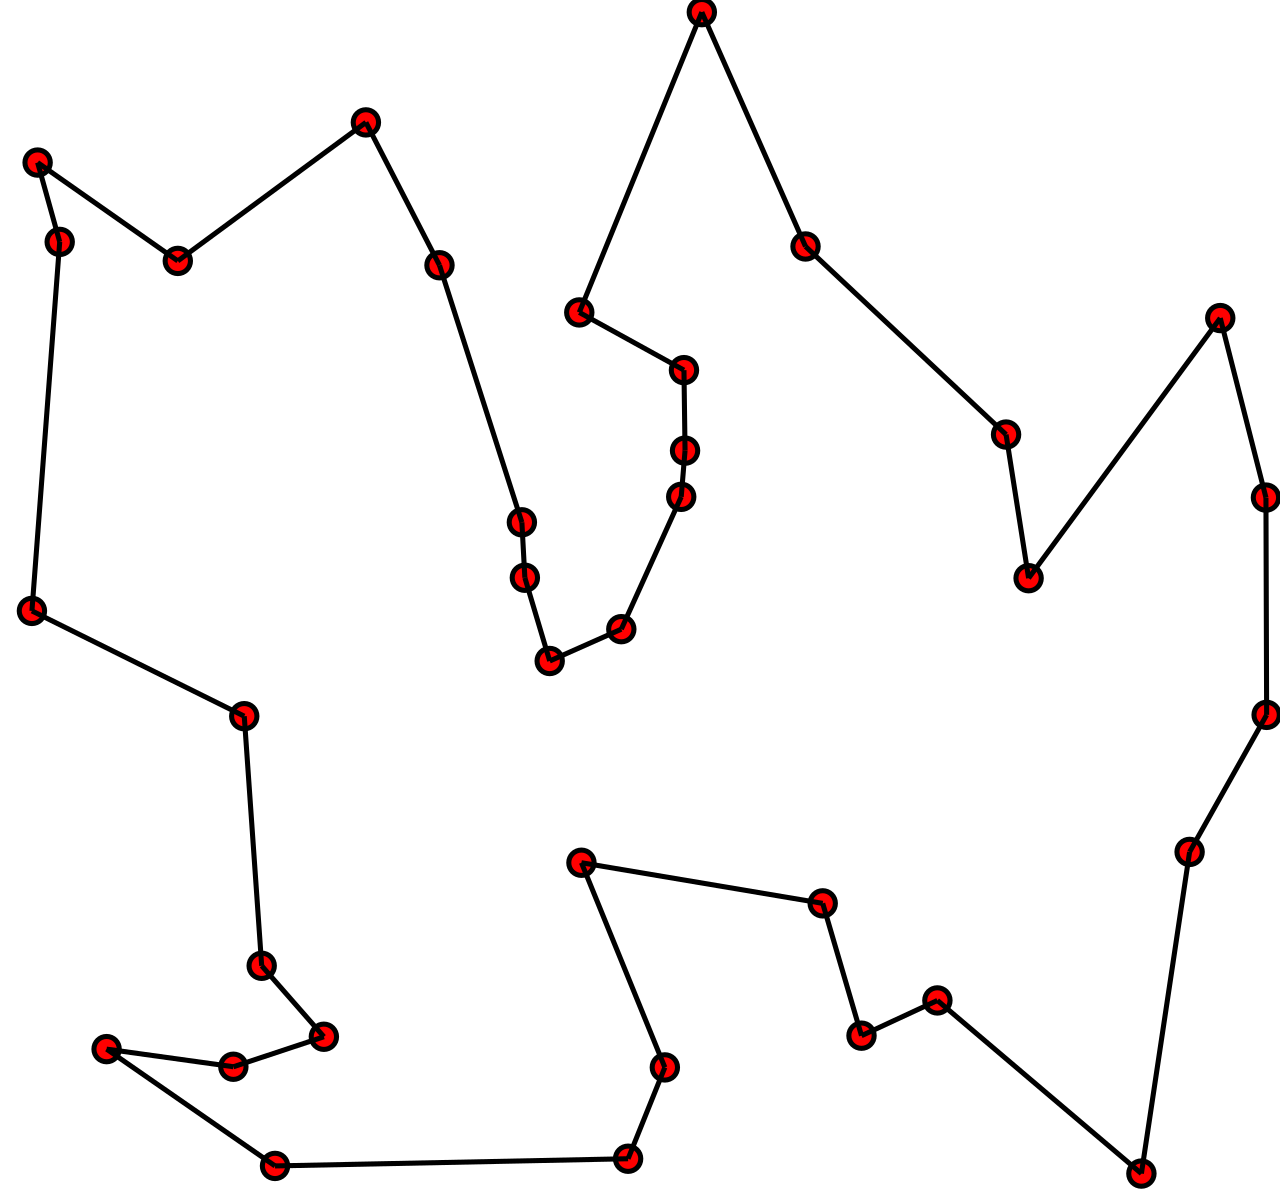
\includegraphics[width=0.4\textwidth]{solution_of_a_TSP.png}
    \end{center}
    \caption{\label{fig:solution_of_TSP} A solution example for TSP. Red points represent locations, lines represent the optimized route.}
\end{figure}

Algorithms to reduce the calculation time are essential. Many heuristic algorithms have been utilized in solving TSP\cite{TSP_review},
for example: ant algorithm, greedy method, simulated annealing, tabu search and genetic algorithm \cite{genetic_on_TSP}. 
The genetic algorithm randomly samples values of the changing cells between lower and upper bounds to generate
a set of combinations of possible routes, and choose the best one.
Genetic algorithms can give a near-to-optimal solution in a relatively short time, but we cannot know how near it can be to the best route.
Ant Colony Optimization algorithm(ACO) is one of the metaheuristic methods for solving TSP, 
it works like observation of real ants, and upon finding food return to their colony while laying down pheromone trails\cite{ACO_on_TSP}. 
The ACO can also get a near-optimal solution to the traveling salesman problem, it's able to find the global optimum in a finite time.
Some improved ACO algorithms have also been proposed like Parallel implementation of ant colony optimization \cite{para_ACO}. 
Christofides algorithm\cite{VANBEVERN2020118} utilizes Minimum spanning tree(MST) to get the approximation solution of traveling salesman problem, 
which guarantees its solutions will be within a factor of 3/2 of the optimal solution length.
Christofides algorithm has the limitation that it can only be applied on the instances where the distances form a metric space (they are symmetric and obey the triangle inequality) \cite{christofides_inbook}.
The simulated annealing(SA) algorithm is a kind of greedy algorithm. It uses randomness as part of its search for the best solution, so it is a stochastic global search algorithm.
The simulated annealing algorithm is good at jumping out of the local minimum\cite{improved_SA}.

Some other research has been extended into the domain of logistics, 
respective extensions are called Vehicle Routing Problem(VRP)\cite{BRAEKERS2016300}, 
VRP not only optimize the distance between two single points
but also optimize the distances between a series of points under different criterion and restrictions. 
Some research extended VRP to green logistics, 
they optimize the fuel consumption and emissions\cite{green_vehicle}.
Marc Schröder and Pedro Cabral\cite{article} build a model to estimate the $CO_2$ emissions for road freight transportation and found eco-friendly routes can yield up to 20\% emissions reduction.
Jiquan Wang\cite{battery_predict} developed an energy consumption prediction algorithm to make route optimization for electric vehicles.

Another way to handle the TSP problem is using the neural network method\cite{SHI2022681}.
Hopfield neural network\cite{Hopfield:1985aa} is the first neural network for handling TSP, 
which converts the objective function into the energy function of a fully connected neural network.
Several research focused on how to improve the Hopfiled method on its convergence\cite{Luo2019DesignAI} and performance\cite{10.1007/s00521-018-3535-9}\cite{improv_hop}.
Graph neural network is also an architecture to solve TSP problem\cite{graph_neural} when dealing with graph data, 
graph data is a complex data structure that a fully connected network hardly deals with.
Neural network with reinforcement learning\cite{vanOtterlo2012} is a kind of method to solve sequential decision-making problems.
From the notable Pointer network proposed Vinyals\cite{vinyals2017pointer} which used an attention mechanism to take attention as a pointer, 
many reinforcement networks based on it were developed such as graph pointer network with reinforcement\cite{ma2019combinatorial} 
and graph point network with negative travel length as the reward signal\cite{bello2017neural}.

The research about finding the shortest path mentioned above usually uses 2D coordinate data format and none of them did the real-world case in Africa area.
The research about route optimization with the deep learning part mentioned above only uses coordinates as the input data format, 
this data format can only reflect the straight-line distance between locations which is not able to reflect the distance of the real-world road network.
In this project, the path planning part is considered with 3D coordinates 
and a small revision is made on the Pointer Network so that it can use the adjacent matrix as input data format to solve the TSP problem on a real-world network.
Snoocode Corporation has designed a route optimization system that works offline on a smartphone and provides 
results 42000 times faster than the conventional method. However, this method only considers a 2D map.
The next step for Snoocode is developing a method that can optimize the route considering land elevation. 
Elevation is a very important factor for electric bikes and bicycles which are the main transportation of delivery companies in Accra.
To be more specific about the function of the route optimization system, suppose there are 20 locations to
give delivery to, the shortest way need to be found so that every location can be delivered. 

For making a system to do 3D route optimization, the problem is divided into four parts: 
\begin{itemize}
    \item Data processing. Existing software for route optimization or path planning now only uses 2D road data.
          And the coordinates of available open-source road data are in 2D format.
          So the first important task is integrating 2D road data and raster elevation data into 3D road data.
    \item Building 3D road network with processed data. 
          For a real-world road system, it is not correct to do route optimization only with coordinates(straight-line distance) of several locations.
          Because of the complex road conditions, it is impossible to walk in a straight line.
          So a network graph that can easily calculate the shortest distance of any pair of locations is the key.
          With the network, the adjacent for any number of locations can be created for doing route optimization.
    \item Route optimization. This part contains two methods, 
          one is a conventional algorithm(Work of Rutvji Kulkarni: rutvij.kulkarni22@imperial.ac.uk), 
          and the other one is using a deep learning model. 
          Traditional algorithms can achieve a relatively higher efficiency for route optimization than the brute-force method.
          However, as the number of target locations to optimize grows, the computing time grows as well.
          When the number of optimized locations reaches a certain level, even mature algorithms take a long time to optimize.
          A deep learning model to predict the optimized route for a large number of locations can handle this.
          Although it may take a very long time to train the model, 
          SnooCODE can integrate it into the offline mobile application to do route optimization in a short time once it is trained.
          The model architecture used in this research is called Pointer Network developed by Google.
\end{itemize}

\subsection{Code structure}
The codes in this research are developed by Python and encapsulated into several classes based on their functionality.
The structure of the codes is as shown in Fig~ \ref{fig:code_struc.}.
The Road\_network class is the main class for integrating 2D road data with elevation data and creating road network graphs.
There are also some small functions in this class, 
for example: 'get\_data\ function' to get the data stored in the class, 
'get\_shortest\_path' function to return all nodes on the shortest path between two locations,
'get\_shortest\_path\_length' function to get the length value of the shortest path between two locations,
'weight\_matrix' function to get the adjacent matrix given a list of locations. 

The Visualisation class is the class for visualizing the path planning between any pair of locations.
This class also have some functions to show 3D road map and 2D road map.

The City class is for storing the coordinates of locations. There is a coordinate transformation function in the City class, 
If the user inputs a coordinate in latitude and longitude, it will automatically transform it into easting and northing format 
which is easier for calculating distance.

Besides the codes drawn in the code structure figure, 
there is also a class storing loss functions for calculating distance/travel time while creating a network,
a code script for generating a dataset and a Jupyter notebook containing codes to train the deep learning model.
\begin{figure}[H]
    \begin{center}
        \includegraphics[width=1\textwidth]{code_structure.jpg}
    \end{center}
    \caption{\label{fig:code_struc} The code structure. The dark grey block is class, the light grey block is a function, the blue block is data.}
\end{figure}
\section {Methods}
This project mainly focuses on real-world road networks, 
but it is hard to consider all the factors of roads because of their complexity.
Some assumptions are raised in this research:
\begin{itemize}
    \item The ratio of traffic to capacity is 0.5 for all road segments.
    \item There is no traffic light on the road.
    \item Vehicles travel at the maximum speed specified for each road segment with no traffic congestion in consideration.
\end{itemize}
\subsection {Integrate data for 3D road data}
The target city of this research is Accra, Ghana, whose range of coordinates is 5.52N to 5.68N in latitude and 0.31W to 0.01E in longitude.
The main essential data needed in this research are the 2D road information data and the elevation data. 

The 2D road information data was retrieved from OpenStreetMap by Overpass API, whose last updated time is 2023-06-11T03:07:17Z.
The 2D road data is a JSON file, the main part of the data is in key 'elements', and the value of 'elements' is a list containing all road segments in the Accra area.
Each element of the list 'elements' is a road segment, containing keys 'nodes', 'geometry', and 'tags'. 
The value of the key 'nodes' is a list containing several integer numbers that refer to the unique ID of a point, 
The value of the key 'geometry' is a list containing several dictionaries, each dictionary contains 'latitude' and 'longitude' which refer to the geographical coordinates of a point.
In each road segment, the length of 'nodes' is equal to the length of 'geometry', because the elements in 'nodes' correspond one-to-one with the elements in 'geometry' with the same index.
Connecting the series of points within each element forms the road segment.

The value of the key 'tags' contains the attribute of each road segment, for example: 'highway' is the type of road segment, and 'oneway' indicates whether the road segment is one-way direction.
Fig.~\ref{fig:accra_road} shows the road type distribution of Accra, and Fig.~ \ref{fig:accra_access} shows the access distribution of Accra. 
The road type of road segments has a significant influence on the travel time calculation in a later chapter as there are different speed limits for different road types.
The access type determines whether a road segment can be used for delivery. The attribute 'oneway' is also considered in this research, and road segments that are 'oneway' can only be used in one direction.
\begin{figure*}[htbp]
    \centering
    \begin{minipage}[t]{0.48\textwidth}
    \centering
    \includegraphics[width=7cm]{Roadtype.jpg}
    \caption{\label{fig:accra_road} The road types of Accra. X-axis: road types of Accra, Y-axis: the quantity of each type.}
    \end{minipage}
    \begin{minipage}[t]{0.48\textwidth}
    \centering
    \includegraphics[width=7cm]{AccessType.jpg}
    \caption{\label{fig:accra_access} The access types of Accra. X-axis: access types of Accra, Y-axis: the quantity of each type.}
    \end{minipage}
\end{figure*}

The elevation data is SRTM 1 Arc-Second Global retrieved from the website USGS. The elevation data is in raster format, whose resolution is about 30 meters/pixel. 
The integration of 2D road data and elevation data is to add one key 'ele' in the key 'geometry' for each point in the 2D road JSON file, which represents the elevation of that point. 
Because the elevation data is a raster data and each pixel of elevation data is in the shape of $30m*30m$, 
there might be some different road points in the same grid. 

To make the integration of these two data more precise, interpolation is applied so that every road point is assigned its elevation value according to the values of the four pixels surrounding it.
The schematic diagram of interpolation is shown in Fig.~\ref{fig: interpolation}. The process of interpolation is as follows:
\begin{figure}[H]
    \centering
    \includegraphics[width=0.5\textwidth]{interpolation.jpg}
    \caption{Illustration of interpolation. Grids represent pixels of raster elevation data. Black points represent the center of grids. A, B, C and D represent four grid centers surrounding target red point P. The red dashed line divides grid D into four sub-grids. Red double arrow lines represent the distance between A, B, C, D and P.}
    \label{fig:interpolation}
\end{figure}

\begin{enumerate}
    \item Get the grid length $l$.
    \item Find the current grid the point $p$ belongs to.
    \item Find which subregion of the current grid the current point $p$ belongs to.
    \item Use the elevation data of four grids surrounding the point $p$ to interpolate the elevation. In this diagram, $(i-1,j-1)$, $(i-1,j)$, $(i,j-1)$, $(i,j)$.
    \item Calculate the weight for the point $p$. For example: the weight of point $A$ is: $w_A = 1/distance(p, A)$
    \item Calculate the elevation of point $p$ with the following equation:
    \begin{equation}
        h_p = \sum_{i=1}^{4}\frac{w_i h_i}{\sum_{i=1}^{4} w_i}
    \end{equation}
\end{enumerate}

The calculated elevation of each point is added in the 2D road JSON file as the key 'ele' in the key 'geometry'.
After this process, the 2D road data is turned into 3D road data.

\subsection{Building 3D road network}
To easily calculate transportation indicators like distance, and travel time between any two pairs of points in Accra, building a 3D road network is essential.
In this research, a 3D road network graph is built by the open-source package NetworkX based on the integrated 3D road data.
The transportation road network graph consists of nodes and edges, nodes are points in the 3D road data and edges are formed by sequentially connecting the points of each road segment.   
Every node will be assigned a unique ID while creating, which is the same ID in the 3D road data file.

The one-way road is considered based on the attribute 'oneway' in the 3D road data when creating an edge.
If the road segment is a one-way road, the edges of this segment are created only once in the given sequence. 
However, if the road segment is not a one-way road, the edges of this segment are also created in reverse order.
As a consequence, if the road is not one-way, there will be two-directional edges in opposite directions between two nodes in the segment,
if the road is one-way, there will only be one-directional edge between two nodes in the segment.

When creating edges for each road segment, each edge would be assigned with some attributes, like distance and travel time.
Users can also define their own attributes like battery consumption in the class 'CostFunctions'. 
The distance attribute is calculated based on the following equation:
\begin{equation}
    distance(i,j) = \sqrt{(x_i-x_j)^2 + (y_i-y_j)^2 + (z_i-z_j)^2}
\end{equation}
where $i$ and $j$ indicate two different nodes, and $x$, $y$, $z$ indicate the coordinates of a node.
The travel time attribute is calculated based on the following equation:

\begin{equation}
    T_i = T_i^0(1+\alpha(v/c)^\beta)+Gradient_i
\end{equation}

\begin{equation}
    Gradient_i = \frac{G_.D_.}{S_i} \times P_i(P_i>0)
\end{equation}
where $T_i^0$ is the free travel time of the road segment; 
$v/c$ is the ratio of traffic to capacity, based on the assumption mentioned before, this value is 0.5 for all road segments;
$\alpha$ and $\beta$ are two parameters ($\alpha=0.15, \beta=4$); $G_.D_.$ is the road segment length with a slope;
$S_i$ is the free flow speed of the road segment; $P_i$ is the slope weight of the road segment. 

The free flow speed of different road segments is on the road type, as shown in Table \ref{tab:speed_limit}.
\begin{table}[H]
    \centering
    \begin{tabular}{|c|c|}
    \hline
    Road type & Speed limit (km/h) \\
    \hline
    Primary & 50 \\
    Secondary & 50 \\
    Tertiary & 50 \\
    Trunk & 50 \\
    Residential & 20 \\
    Motorway & 80 \\
    Service & 20 \\
    Unclassified & 50 \\
    \hline
    \end{tabular}
    \caption{\label{tab:speed_limit}Speed limit of different road types}
\end{table}
    
This network can be used to calculate some information between any pairs of points in the graph.
Information including distance, and traveling time. This information can be added according to the purpose of the user.
After creating the network graph, users can use it to get the best path between any pairs of locations in Accra based on the cost function they choose.
The algorithm to achieve this functionality is the Dijkstra algorithm which is built-in in the NetworkX package.

In this research, I implement a function that can output the adjacent matrix based on the input of a list of locations.
Each entry of the adjacent matrix represents the cost between the corresponding pair of locations. 
This function is the most important part of generating data to train the deep learning model for the TSP problem of a real road network.

\subsection {Pointer Network for TSP problem of 3D road network}
The deep learning model architecture used in this research is Pointer Network\cite{vinyals2017pointer}.
The Pointer Network's structure as shown in Fig.~\ref{fig:pointernet} uses one encoder to receive and transcode the adjacent matrix data into the hidden layer.
Then it uses a decoder and an attention mechanism to calculate the mechanism score with the hidden layer of the encoder.
The mechanism score is used to produce the pointer or index of the next location to go.
\begin{figure}[H]
    \centering
    \includegraphics[width=0.8\textwidth]{Pointer_network.jpg}
    \caption{\label{fig:pointernet}Illustration of pointer network. Ptr-Net - An encoding RNN converts the input sequence to a code (blue) that is fed to the generating network (purple). At each step, the generating network produces a vector that modulates a content-based attention mechanism over inputs ([5, 5]). The output of the attention mechanism is a softmax distribution with a dictionary size equal to the length of the input. The input at each step is an entry of the adjacent matrix.}
\end{figure}
The decoder is a masked LSTM model, after a location is predicted in a time step, the pointer for this location will be masked.

To train this model, a 70000 dataset is generated. Each data point contains one adjacent matrix and one label.
The adjacent matrix is of five different random locations in Accra, the entry of the adjacent matrix is calculated by the distance cost function,
and the label is the optimized route for these five locations in a format of the list of indices.
The optimized route for each data point is calculated by brute-force algorithm, so it can be sure that the route is the optimal solution.

The model is trained for 5000 epochs, with the 2048 batch size.


\section {Results}
\subsection{Performance of Integration}
The tool developed in this research shows that route optimization performance for any two locations in Accra
is close to Google map's performance.
The visualization of the path done by this tool is shown in Fig. ~\ref{fig: mine}.

\begin{figure}[H]
    \centering
    \includegraphics[width=0.7\textwidth]{kotoka_uni_mine.jpg}
    \caption{\label{fig: mine} Path from Kotoka airport to University of Ghana by this research. Black lines are streets. Red lines are the shortest path. Colors represent elevation.}
\end{figure}
The corresponding path planning done by Google is shown in Fig. ~\ref{fig: google}. 
It can be seen that the travel paths are almost the same in this case.
\begin{figure}[H]
    \centering
    \includegraphics[width=0.4\textwidth]{kotoka_uni_google.jpg}
    \caption{\label{fig: google} Path from Kotoka airport to University of Ghana by Google.}
\end{figure}

To verify the performance of the tool developed in this research, 
the optimized paths of 100 random pairs of locations are compared with the paths from Google Maps for the same 100 pairs of locations.
The relative mean squared error(RMSE) is calculated for the 100 random paths is calculated.
To verify the distance cost function, walking is chosen for transportation in Google Maps as this is the way to get the shortest way.
To verify the time travel cost function, driving with a clear road is chosen for transportation in Google Maps as this is the way to get the least time-consuming path.

Five sample pairs locations for testing are as follows:
\begin{enumerate}
    \item Kotoka International Airport - University of Ghana
    \item Kotoka International Airport - Accra zoo
    \item Kotoka International Airport - National Museum of Ghana
    \item Accra Zoo - University of Ghana
    \item Accra Zoo - National Museum of Ghana
\end{enumerate}

\begin{table}[H]
    \centering
    \begin{tabular}{|c|c|c|c|c|c|c|}
    \hline
   case & distance & distance(Google) & Relative Error & time & time(Google) & Relative Error\\
   unit & km & km &  & minute & minute &   \\
    \hline
    1 & 6.55 & 6.5 & 0.77\% & 12.85 & 13 & 1.15\% \\
    2 & 6.94 & 7.7 & 9.9\% & 14.32 & 15 & 4.5\% \\
    3 & 7.5 & 7.4 & 1.4\% & 13.62 & 13 & 4.8\% \\
    4 & 5.4 & 6.8 & 20.6\% & 12.18 & 22 & 44.6\% \\
    5 & 9.97 & 9.7 & 2.7\% & 18.89 & 21 & 10.04\% \\
    \hline
    \end{tabular}
    \caption{\label{tab:route_results}Route results compare with Google.}
\end{table}
The compared results of five sample paths are shown as Table \ref{tab:route_results}. 
As we can see, the RMSE of distance for 100 random paths is 11.95\%. 
This is a relatively good result, which means that this tool can find the shortest path in most cases.
But there still are some cases that are not the shortest way like case 5.
The reason may be that this tool only finds the effective route of road segments with the 'highway' tag,
so some road segments without the 'highway' tag may be ignored,
the tool has to skip these road segments and use some longer road segments when finding the best route.
What's interesting is that there are some paths found by this tool shorter than the results from Google.
This may be because some road segments can not be accessed but have no 'access' tag in the JSON file, 
so the tool makes it able to be accessed by default. These road segments can be a shortcut which can make the path shorter.

For the travel time part, the tool's result seems to not be good enough.
The RMSE of travel time is 23.73\%, which is relatively high. 
It can be seen from the table that most travel time calculated by the tool is smaller than travel time from Google Maps.
There might be two reasons for that. 
The first reason is the vehicle speed of each road segment in this tool is the max speed limit. 
Although the travel time from Google Maps is also calculated by the condition of clear roads, 
the vehicle speed for calculating travel time does not reach the max speed limit in Google Maps.
The second reason is that Google map considers how long it takes to wait at a traffic light, 
even though the condition of the roads is clear.
Considering these two factors together, the time calculated by the tool can be much smaller than the travel time from Google Maps.
The travel time from Kotoka airport to the University of Ghana seems very close to the travel time from Google Maps. 
The reason for this might be the route from Kotoka airport to the University of Ghana is mainly composed of trunk road segments,
and there are few traffic lights on the trunk roads.
Although the travel time calculation might have deviation from the real-world travel time, 
the path planning by the tool is with reference significance.

\subsection{Performance of Pointer Network}
To evaluate the performance of the trained Pointer Network, two criteria are chosen. 
The first criterion is accuracy. 
The correct answer should make the values and positions of predicted indices all correct.
The second criterion is the route length ratio, 
which is the ratio between the total length of the predicted route and of the true optimized route.
The smaller the route length ratio is, the higher performance the model has, 
and the best route length ratio should be 1.

A test dataset with the size of 70000 is created to verify the performance of the model. 
The result shows that the accuracy of the model is 67.0\%,
and the mean route length ratio is 1.02.
The performance of the pointer network with an adjacent matrix as input shows that 
The model can predict almost the best-optimized route. 
Although the accuracy of the model is less than 70\%, the average route length ratio is very close to 1.
The main reason for the error is that there might be two points that are very close to each other 
or the distance of the two points is close to 0 because the dataset is generated randomly.
The order of two locations that are very close to each other has little effect on the route distance calculation, 
so the model may get confused with this kind of pair of locations and yield a wrong order for the two locations.

\section {Discussion}
In this research, a tool for integrating 2D road data and elevation data into 3D road data is developed.
The main difficult task for this process is how to merge two different types of data.
The 2D road data consists of several road segments, and each road segment consists of several discrete points, 
while the elevation data is raster data with a 30-meter resolution. 
To address this problem, two methods are considered. 
The first one is using the value of the block to which the road segment point belongs. 
This method is simple but cannot handle the case that two points belong to the same grid of elevation data.
The second one is interpolation for each point in the road data. In the tool developed by this research, 
which of the four subregions of the elevation grid each point belongs to should be found first, 
and then values of this grid and the other three grids that are adjacent to the subregion are used to do interpolation.
The weight for doing interpolation is inversely proportional to the distance between the target point and the grid center.
This method is more time-consuming than the first one, but it can achieve a relatively higher precision.

After the integration process, the network for a city is created.
The main difficult task to resolve in this process is how to make an easily used network to do route planning.
The mature method to resolve this task is creating a graph for the road network, which consists of nodes and edges.
Nodes are created from the points in integrated road data, and edges are created by connecting the nodes sequentially.
When creating edges, two cost functions are integrated distance and travel time. 
Users can do route planning based on the cost function they choose. 
The distance cost function can make route planning in the real-world street map which is close to Google Maps.
The limitation in this part is that the travel time cost function is based on several hypotheses, 
such as the road is clear, there is no traffic light, and vehicles go at the maximum speed. 
These hypotheses may lead to the calculated travel time deviated from real travel time, 
but it can still be used to give the least time-consuming route.
Another main reason for the deviation is the road data itself. 
The tags of road data collected from OSM may be not enough to reflect the real-world case.
For example, some roads may be only available for pedestrians, and some roads may not be able to be accessed.
This may cause some little error on a small amount of road segment, because some private-access way may be a shortcut.
To improve the performance of this process, data should be refined gradually, which can make the network closer to the real-world case.

After the two processes mentioned before, the dataset can be generated by the tool for training the revised Pointer Network.
The model can not distinguish locations that are close to each other very well, which affects the accuracy of the model.
Despite the relatively low accuracy, the model can still achieve a route optimization that is close to the optimal answer on average.
To improve the performance of the model, 
more data with more complex modes can be fed to the model during training so that the model can learn how to handle these modes.
The original Pointer Network can be extended for predicting optimized routes for more locations than the number of training locations.
But in my revised Pointer Network, the input of the model is changed to the adjacent matrix. 
The strength of this revision is that it can be used for route optimization of the real-world road network.
The limitation of this revision is that it can not be extended to predict the optimized route with more locations than the number of locations during training.
Because the input layer of the model is fixed, the size of the adjacent matrix is according to the number of locations to do route optimization.
To improve this, users can train different models for different numbers of cities, 
or the structure of the model could be improved in the future so that it can adapt to the variable size adjacent matrix.

\section{Conclusion}
In this research, a tool that can integrate 2D road data and elevation data into 3D road data as well as route planning and visualization is developed.
The integration function of the tool can be used on any other area in addition to Accra specified by users. 
The route planning function of the tool can achieve 11.95\% relative error for finding the shortest path,
and 23.73\% relative error for finding the most time-saving path compared to Google Maps.
Using the data generated from the tool mentioned above, 
a revised Pointer Network is implemented to predict the answer of TSP given adjacent matrix, 
which can be used for real-world street route optimization.
The accuracy of the model is 67.0\%, the average route length ratio compared to the optimal route length is 1.02.

% References
\bibliographystyle{unsrt}
\bibliography{references}  % BibTeX references are saved in references.bib

\end{document}          
